
%(BEGIN_QUESTION)
% Copyright 2010, Tony R. Kuphaldt, released under the Creative Commons Attribution License (v 1.0)
% This means you may do almost anything with this work of mine, so long as you give me proper credit

Process chromatographs are {\it multi-variable} instruments, and so analog versions are often equipped with multiple 4-20 mA outputs to transmit concentration data for each measured component:

$$\includegraphics[width=15.5cm]{i00669x01.eps}$$

Inspecting this loop diagram, answer the following questions:

\begin{itemize}
\item{} What is the purpose of the vessel labeled ``He''?
\vskip 10pt
\item{} Do the DCS input cards supply 24 VDC loop power or not?
\vskip 10pt
\item{} How would you connect a loop calibrator to simulate a 50\% signal to AIR-43c?
\vskip 10pt
\item{} Can you think of any way we could reduce the number of cables needed to convey the data from the chromatograph to the DCS?
\end{itemize}

\underbar{file i00669}
%(END_QUESTION)





%(BEGIN_ANSWER)

\begin{itemize}
\item{} What is the purpose of the vessel labeled ``He''? {\it This is the carrier gas tank, filled with helium.}
\vskip 10pt
\item{} Do the DCS input cards supply 24 VDC loop power or not? {\it Most likely not, since the chromatograph has its own 120 VAC power connections, it is most likely the loop power source and not the DCS.}
\vskip 10pt
\item{} How would you connect a loop calibrator to simulate a 50\% signal to AIR-43c? {\it Disconnect cable AIT-43c from either the chromatograph terminals or the DCS input channel terminals, then set the loop calibrator to ``source'' mode (not ``simulate'' mode!) and use it to drive 12 mA of current into the DCS channel.}
\vskip 10pt
\item{} Can you think of any way we could reduce the number of cables needed to convey the data from the chromatograph to the DCS? {\it Use some form of digital communication rather than analog between the chromatograph and the DCS.  One option is multi-drop HART, another is FOUNDATION Fieldbus (or some other fieldbus standard such as Profibus).  Another option yet is to remote-mount the DCS I/O near the chromatograph, then use the DCS network cable to bring the data to the main control room.  A similar option would be to remote-mount a PLC near the chromatograph, then run a network cable from the PLC to the DCS, possibly using a ``bridge'' device to translate the PLC's network protocol into a form the DCS can interpret.}
\end{itemize}

%(END_ANSWER)





%(BEGIN_NOTES)


%INDEX% Measurement, analytical: chromatography

%(END_NOTES)

